\chapter{QuickStart}%
\label{cha:Quickstart}

\section{Cinelerra-GG Quick Start Guide}%
\label{sec:cin_quick_start_guide}

Cinelerra is a software program NLE, Non-Linear Editor, that provides a way to edit, record, and play audio or video media on Linux.   It can also be used to color correction, retouch photos, motion tracking, watch TV, and create DVDs.

\subsection{Install the Software}%
\label{sub:install_software}

On the internet, click on the Download page at:  \quad {\small \url{https://cinelerra-gg.org/downloads/}}
Here you will see several Operating System distro packages that are already built for you to download.  Click on your preference and read the specific instructions for usage.

\begin{figure}[htpb]
	\centering
	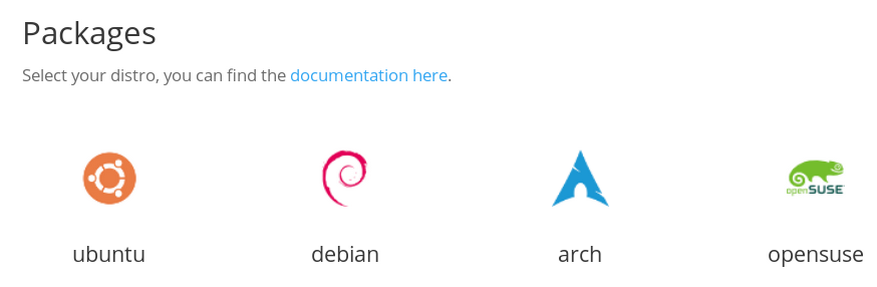
\includegraphics[width=1.0\linewidth]{images/packages.png}		
\end{figure}

However, if you want to get going as quickly as possible, just do this so that everything is in 1 place:

\begin{itemize}[noitemsep]
	\item Download your Operating System’s tar file from {\small \url{https://cinelerra-gg.org/download/tars/}} to \texttt{/tmp}.
	\item Key in:  cd /name-of-directory-where-you-want-the-software (for example, \texttt{cd /software})
	\item Key in:  \texttt{mkdir cin}
	\item Key in:  \texttt{cd cin}
	\item Key in:  \texttt{tar -xJf /tmp/cinelerra-5.1-*.txz}   (if you put the tar in \texttt{/tmp} AND replace * with full name)
\end{itemize}

\subsection{Start Cinelerra GG}%
\label{sub:start_cinelerra_gg}

Depending on how you installed the software, you can log in as root or as a user if you used a package.

\begin{itemize}[noitemsep]
	\item Key in:  \texttt{/your-software-directory-path/bin/cin}
	\item Or if you installed using the pkg method, click on the \textit{Cin icon}.
\end{itemize}

You will now see 4 separate windows appear.  The top 2 windows from left to right are the Viewer which is most useful for previewing clips and media and the Compositor which displays the current working frame at the timeline position.  The bottom 2 windows are the Cinelerra Program, also called the timeline, which is where the real work gets done and the Resources window showing a selection of media or effects.

\begin{figure}[htpb]
	\centering
	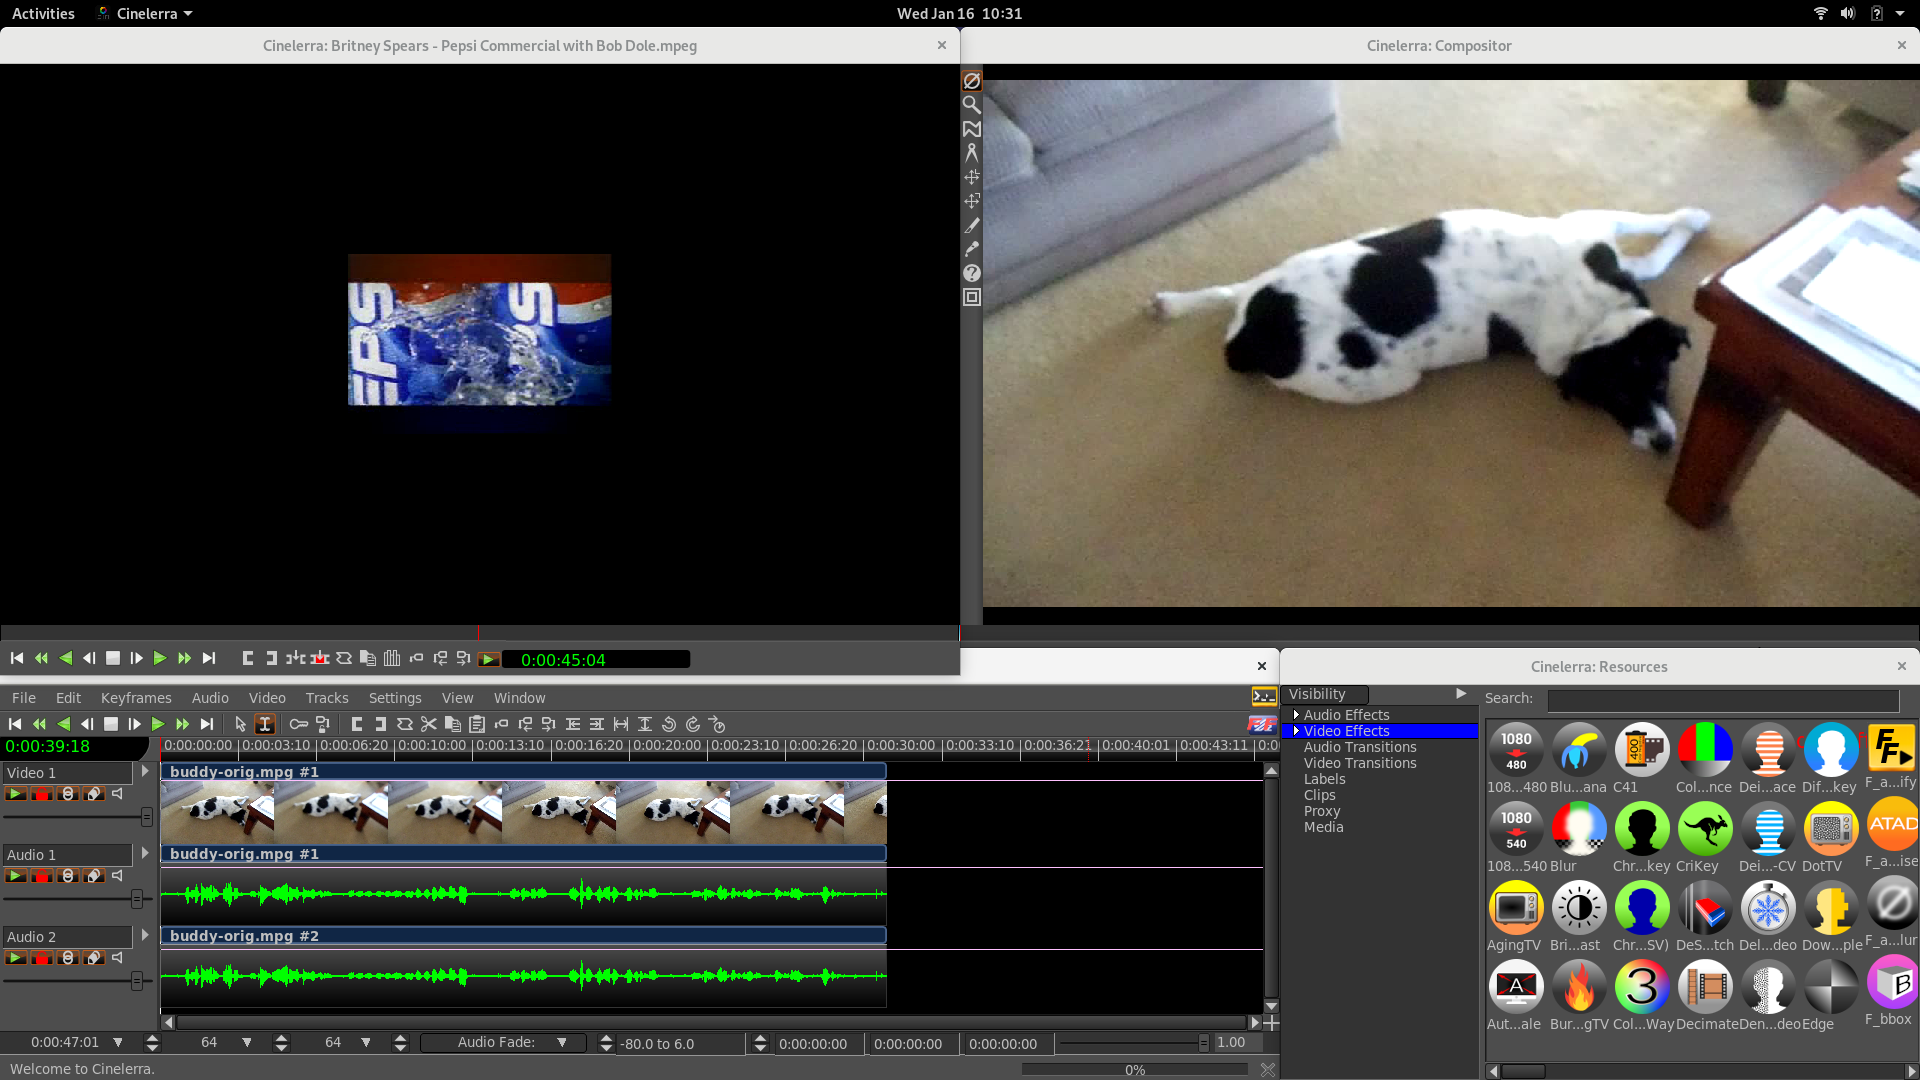
\includegraphics[width=1.0\linewidth]{images/4windows.png}
	\caption{Clockwise: Viewer; Compositor; Resources and Main/Program/Timeline}	
\end{figure}

Any of these windows can be resized to better suit your needs.  Note that if your system’s native language is not English, some of the words you see on the screen will be correctly translated for you, others will be in english, and some will have not very good translations.

It is important to know that Cinelerra does not directly change your media.  It writes all changes to what is called the EDL, Edit Decision List.  This way you original media remains completely intact.

\subsection{Load Media}%
\label{sub:load_media}

On the main timeline program window are many pulldowns, the first of which is \textit{File}.

\begin{figure}[htpb]
	\centering
	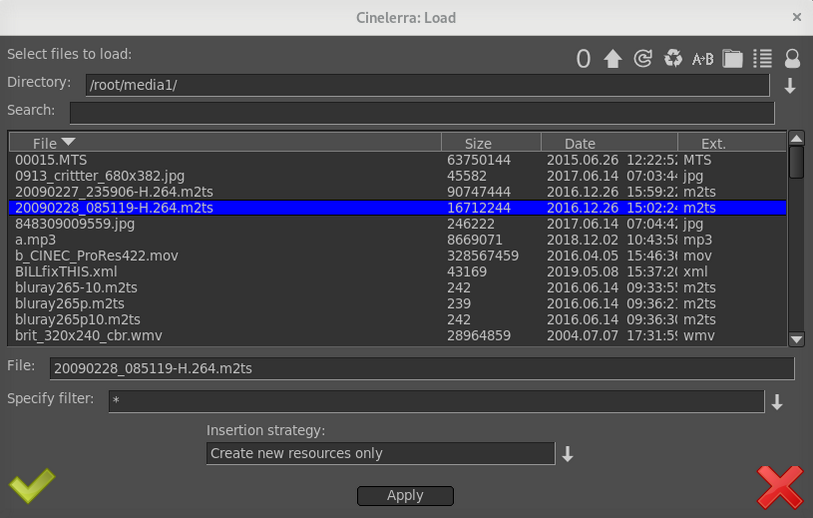
\includegraphics[width=1.0\linewidth]{images/load_files.png}
	\caption{Load media window -- note the icons top right for more options}	
\end{figure}

\begin{enumerate}
	\item Click on \texttt{File} for a list of available options and note that in the right hand column are shortcuts for
	many of the options that will come in handy if you use Cinelerra often.
	\item Next click on the second one down -- \texttt{Load files$\dots$} -- which brings up the Load menu.
	\item Below \texttt{Select files to load} on the top left side is a textbox and if you look all the way to the right
	side of the textbox, there is a down arrow which you use to navigate your file system.  Highlight the
	desired file system and you will see that directory name appear in the textbox and the files below.
	\item Scroll to the media file you would like to work on and highlight that file.  When you do, you will
	see that filename also appear in the textbox below the listing of files.  You could have directly
	keyed in that file in that textbox instead.
	\item On the bottom of the Load menu, is a box called \textit{Insertion strategy}.  For getting started the
	default of \texttt{Replace current project} is sufficient.  But you can click on the down arrow to see what
	is available for future use.
	\item Now click on the green colored checkmark on the bottom left hand side to actually load the file
	and see it appear on the timeline in Cinelerra’s main window and a single frame in the Compositor.
	The first track will most likely be video thumbnails and the next tracks may be audio waveforms.
	\item Press the space bar in the main Program window and your video will start playing and press the
	space bar again to stop the play.  While playing, you should see the video in the Compositor
	window in the upper right hand side of your screen and if you have your audio hooked up, you
	will hear the sound.  To get back to the beginning of the video, hit the home key on your keyboard.
\end{enumerate}

\subsection{Choose Output Format}%
\label{sub:choose_output_format}
	
You can skip this step if you want the format of your output to be the same as your input.  However, to create output media that is widely viewable on many platforms, to include phones and television, you should set your format accordingly.

\begin{enumerate}
	\item On the main timeline, use the \textit{Settings} pulldown (about the $7^{th}$ pulldown from the left side top) and
	click on \texttt{Format} which is the first option in that list.
	\item A \textit{Set Format} menu will appear that shows what the current format is for your loaded media in an
	Audio and a Video tab.  In the United States, the Video Frame rate is usually expected to be 29.970	and usually the Color model is only changed if you have a personal preference.
	\item The \texttt{Canvas size} is probably the only thing you will want to change here in order to get to the
	most commonly viewable settings.  On the right hand side of the Width parameter is a down arrow. 
	Left click the down arrow to see your options.
\end{enumerate}

\begin{figure}[htpb]
	\centering
	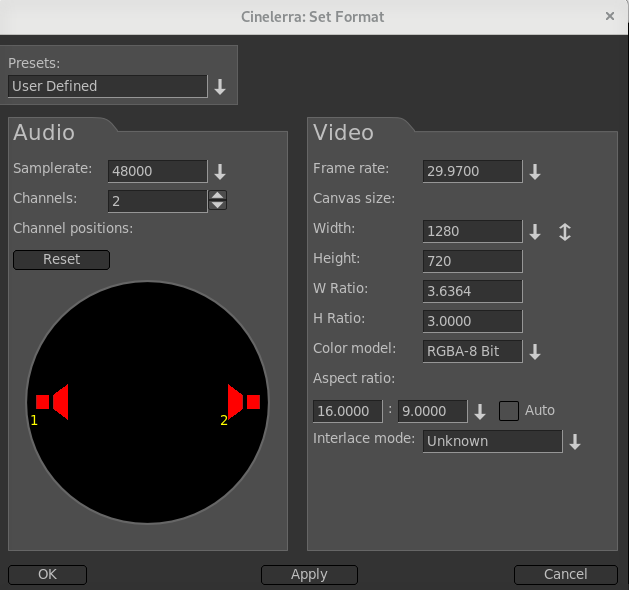
\includegraphics[width=0.8\linewidth]{images/format_setting.png}
	\caption{Format menu to change settings}	
\end{figure}

\begin{enumerate}[resume]
	\item Highlight $1280\times720$ HD for a good common option.
	\item Click \texttt{OK} to have this option take effect.  When you do, the Compositor window may change to fit
	this option and may look wrong sized.
	\item If the video now looks too small or too large in the Compositor, you will want to \textit{autoscale} it to
	look correct when the new media is created.  To do this, mouse over to the Resources window in the
	lower right hand corner and under the word Visibility, highlight \textit{Video Effects} to see some
	plugins.
	\item Mouse over the \textit{Auto Scale} icon, left click to highlight the words underneath the icon, and mouse
	drag the icon to the timeline video track.  When you see a white colored outline show on that track,
	drop the Auto Scale icon there and you will see that the video may now automatically scale to a
	new value.  Click on the magnifying glass icon on the brown colored line beneath the main timeline
	video which opens a new window.  In that window, again use the down arrow to choose $1280\times720$
	HD, then dismiss this window.
\end{enumerate}

\begin{figure}[htpb]
	\centering
	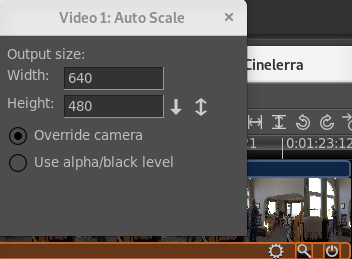
\includegraphics[width=0.6\linewidth]{images/magnifier.png}
	\caption{Effect brown bar with magnifier}	
\end{figure}

\begin{enumerate}[resume]
	\item If not needed, to remove the Auto Scale plugin, right mouse on the brown line and choose \texttt{Detach}.
\end{enumerate}

\subsection{View and Listen}%
\label{sub:view_listen}

\begin{figure}[htpb]
	\centering
	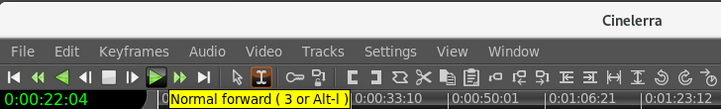
\includegraphics[width=1.0\linewidth]{images/pulldown_button.png}
	\caption{Menu pulldowns at the top with Transport buttons below.  Note the yellow tooltips too.}	
\end{figure}

\begin{enumerate}
	\item On the second line, below the pulldowns, are transport buttons to move back and forth on the
	timeline and play forward or reverse, fast or slow, or a single frame.  When you mouse over one of
	these buttons, a yellow colored tooltip appears to tell you its function along with a key shortcut
	inside of parenthesis.  When you left click the mouse on the transport button it starts the play and 
	click again to stop it.  As you use these buttons, watch the Compositor to watch your video.
	\item On the timeline, you only see thumbnails and not every single picture.  You may want to
	use your keyboard’s \textit{down arrow} to expand the thumbnails and the \textit{up arrow} to unexpand them -- on
	United States keyboard, the arrow keys are generally together on the lower right hand side of the
	keyboard, a little to the right of the space bar.  This is a more cpu intensive operation and for very
	large video can be time-consuming.
\end{enumerate}

\subsection{Edit/Compose}%
\label{sub:edit_compose}

There may be sections of your media that you want to delete, or audio that is hard to hear and needs to be enhanced, or there is a need for a descriptive title that you want to add.  Here are a few basics.  But first be sure that you are in \textit{cut and paste} mode (this is the default) by checking to verify that you see a gold color around the “I” i-beam mode icon as in the figure above.  If the arrow to the left is gold, you are in \textit{drag and drop} mode so switch to \textit{cut and paste} by clicking on the “I” instead.

\begin{figure}[htpb]
	\centering
	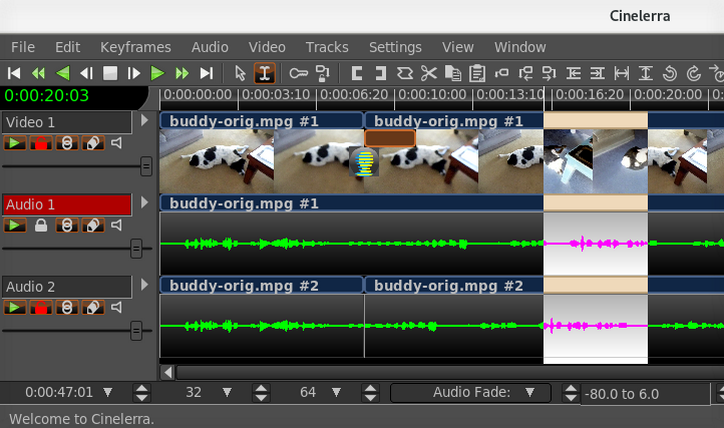
\includegraphics[width=1.0\linewidth]{images/some_editing.png}
	\caption{From left to right:\textit{ Audio 1} is disarmed --  BandSlide transition in \textit{Video 1} -- A highlighted section.}	
\end{figure}

\begin{enumerate}
	\item You should look at the \textit{Edit} pulldown - $2^{nd}$ from the upper left on the main timeline to see the
	most common options to use.  The first option in the list is \texttt{Undo} followed by a terse comment of  
	the last operation that you performed that can be undone.
	\item To delete a section of video/audio is described next.  Various ways to do that are available but the
	easiest is to move your mouse and left click at the beginning of the section you want to delete on the
	timeline and while holding down the left mouse button, drag to the end of the section to be deleted. 
	When you do this, a white colored highlighted section becomes visible.  Use the edit pulldown and
	choose the \texttt{split/cut} option to cut out the highlighted area (note the shortcut of \texttt{x}).  Remember if you
	cut the wrong thing out you can always use the Edit pulldown to Undo that.
	\item To add a transition where there is deleted section which may make your video look disjointed, do
	the following.   Go back to the Resources window in the bottom right hand corner.  Change to
	\textit{Video Transitions} by highlighting that underneath the word \textit{Visibility}.  Highlight a transition like
	\texttt{BandSlide} with the left button mouse click, hold down and drag to the video track and when you see
	a white colored box around the area that you deleted above, drop the icon.  Right mouse click the
	icon on the track to vary some parameters like length.
	\item  To insert another clip from a different video, first you have to load the other video on another track.
	Go to \textit{File} pulldown again and choose the \texttt{Load files} option.  Type in a directory at the top again and
	erase any specific file that you may have chosen previously in the bottom 2 textboxes.  It is very
	important to now change the Insertion strategy to \texttt{Append in new tracks} or you will write over
	your current work.  But if you make this mistake, you can use the Edit pulldown and Undo that!
	\begin{enumerate}
		\item Once the new video is on the track below your current work, you want to work with only this new 
		track, so disarm your other tracks by looking to the left of each track’s timeline and click the $2^{nd}$ 
		button beneath the track name, for example Video 1 or Audio 1.  The track name textbox will turn
		red to remind you that the track has been disarmed.  The boxed area is called the patchbay.
		\item Move to the area you want to make a clip of on your newly loaded track, hold down the left mouse
		button and drag the area to be made into a clip which will turn the color white.  Remember, you
		disarmed the other tracks so only this track is relevant at this time.  On the second line of the main
		window to the right of the transport buttons, are action buttons and as you mouse over them a
		yellow colored tooltip explains its purpose.  Find the one that says \textit{To clip} which is on the right
		hand side of the right bracket symbol.
		\item Click on \texttt{To clip} and a small window comes up which you can comment in, but you do not have
		to, so just click on the green checkmark and now you will have a clip.
		\item Disarm that new track and re-arm your original tracks so you can go back to working on them
		\item Move your cursor to the spot in your original video where you want to insert the clip.   Make a
		\textit{Split} with the \texttt{Split | Cut} option.
		\item Go to the Resources window and under the word Visibility, highlight \textit{Clips} so you can see your
		recently created clip in the box to the right.  Highlight that clip and drag it to where you did the
		blade cut and drop it in.
	\end{enumerate}
\end{enumerate}

\begin{figure}[htpb]
	\centering
	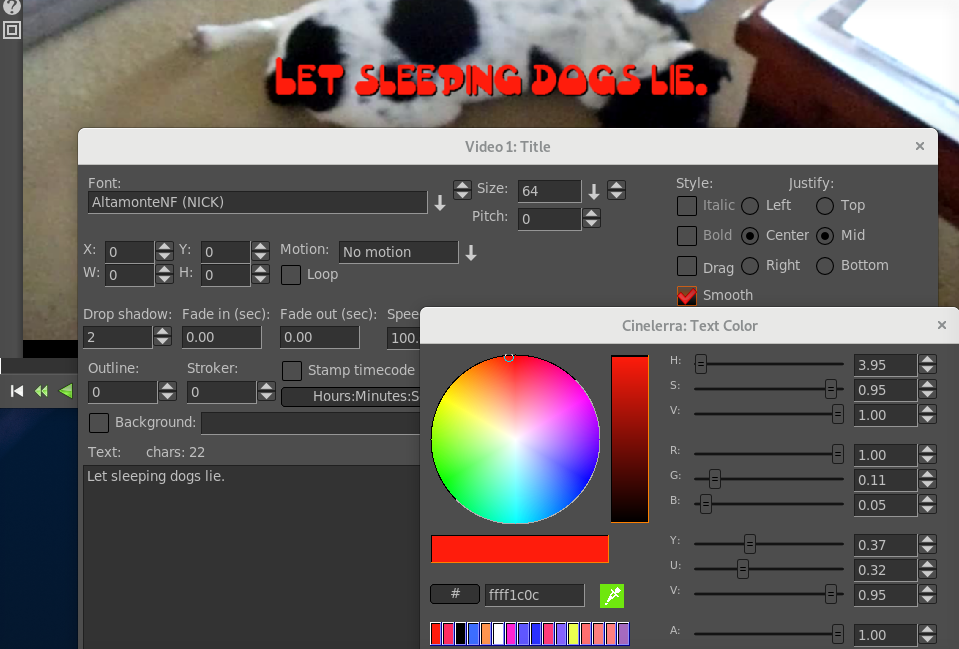
\includegraphics[width=1.0\linewidth]{images/title_color.png}
	\caption{Compositor + Title menu for setting parameters + the Color Picker.}	
\end{figure}

\begin{enumerate}[resume]
	\item To add a Title or any wording you will use the \textit{Title} plugin.  In the Resources window, under the
	word \textit{Visibility}, highlight \textit{Video Effects}.  In the box to the right, many plugin icons appear.   Scroll
	to the right using the scroll bar at the bottom of the Resources window to locate Title.  Highlight the
	\textit{Title} icon and drag/drop to your video track.  By now your video track may be in sections as you
	deleted, added blade cuts, and inserts so where you drop the Title icon will be surrounded with a
	white colored box.  It will take effect in that entire area so you may want to highlight a section as
	usual with left mouse click on the timeline and drag to the end of the desired area.
	\begin{enumerate}
		\item Right click on the brown colored bar that appeared below your video track to get to options and
		then left click on \texttt{Show} to get the Title window to appear.
		\item Now for the fun part.  First type in some words in the bottom large text box just to see what it
		does.  There are so many variable parameters here and they are a lot of fun to play around with.
		\item You can dismiss the Title window when finished BUT be sure to leave the brown colored Title bar
		on the track.  And if you enabled the “drag” feature, you should disable it so you do not forget.
		\item Right mouse click on the bottom Text box to see many more interesting parameters.
	\end{enumerate}
\end{enumerate}

\subsection{Back up your work}%
\label{sub:backup_your_work}

At this time, or even earlier if you think you might make a mistake or if you are concerned about computer crashes, you should save your work.  Use the \textit{File} pulldown, and you can use \texttt{Save as} to designate a directory and filename.  Then click the green checkmark.  You are saving the EDL which is the set of changes that you have made -- this file is separate from your original media.

\subsection{Create your new media}%
\label{sub:create_new_media}

\begin{enumerate}
	\item Once again in the main Program window, click on the \textit{File} pulldown and highlight/click the \texttt{Render}
	option which is about the $9^{th}$ option down from the top of the list.  A Cinelerra Render menu will
	appear.
	\item First key in the first textbox the file to render to under \textit{Select a file to render to}.
	\item For the \textit{File Format}, click on the down arrow and select FFMPEG (because this is the most
	commonly used format; later you may want to experiment with others).  To the right of that box,
	click on the down arrow and highlight \texttt{mp4} -- again because this is common.  When you click on 
	mp4, notice that if there is an extension to your filename in the \textit{file to render to} above, it may
	change it to mp4 and if there is none, it will add \texttt{.mp4} because that is what is expected.
	\item Make sure there is a red colored checkmark next to the words Audio and Video right below if you
	have/want both audio and video.  To the left of that checkmark box, is a symbol that looks like a
	wrench.  Click on this for Audio just to see the default Preset options which are just fine so dismiss
	the menu.  Then click on the wrench for Video and check Pixels by using the down arrow to the
	right to be yuv420p -- this is most commonly usable option.  And click on the green checkmark.
	\item Check the Insertion Strategy in the Render Menu window.  You might want to change that to
	a different strategy than the default of \texttt{Append in new tracks}.  If not, then when the Render is done,
	your new video will automatically be loaded in another set of tracks below your work tracks.  Click
	on the green checkmark in the lower left corner to start the render.
	\item As the render is running, you will see the video play by in the Compositor.  Rendering is usually
	slow, especially with plugins added.
\end{enumerate}

\subsection{Play your new media}%
\label{sub:play_your_new_media}

The file you created in the Render step should now be playable.  You can test this in Cinelerra most easily by going to the Resource window in the lower right corner, clicking on the Media folder, and dragging and dropping the last video to the Viewer window.  There is a separate set of transport buttons on the bottom on that screen to use for playing.

\section{YouTube with Cinelerra}%
\label{sec:youtube_with_cinelerra}

To create a youtube or dailymotion video, you can easily follow the steps below.  You will have to learn a lot more about Cinelerra to take full advantage of its capabilities and make some really special videos, but this is just to get a start and to see the possibilities.

\begin{enumerate}
	\item Start Cinelerra; usually you can do this by clicking on Cinelerra icon or key in \texttt{{cin\_path}/bin/cin}.
	\item In the Program window on the lower left side of your screen, left mouse click the \textit{File} pulldown.
	\item You will see \textit{Load files} as the second choice so left mouse click this and find your video file to
	load, highlight it, and check the green checkmark in the lower left hand corner to get it loaded.
	\item Edit your video in the Program window using the basic commands of:
	\begin{itemize}
		\item play and then stop using the space bar
		\item move the mouse and then left click to move the insertion (location) pointer
		\item cut a section out by holding down the left mouse and drag, then key in “x” to cut or “c” to copy
		\item paste a copy or cut section by moving the insertion pointer, then key in “v”
	\end{itemize}
    \item Add a title by highlighting the \textit{Video Effects} in the right hand side Resources window; then
    highlighting the \textit{Title} icon and dragging it to the Program window video track and dropping.
    \item Click on the middle icon button (looks like a magnifying glass) on the brown colored Title bar to
    bring up the Title window bottom text box and key in a title.
    \item Use the \textit{File} pulldown to select \texttt{Render} to create the desired video.  In the \textit{Render} window just next to the empty box to the right of the \texttt{ffmpeg} file format, click on the down arrow shown there
    to see the choices and pick \texttt{youtube}.  Then move back up to key in the path and filename to render
    to.  It will pick all of the defaults automatically for you so then just click on the green checkmark to
    have it start.  There is a progress bar in the main window, very bottom of the right hand side.
    \item Key in “q” in the main window to get out of Cinelerra and yes or no to save your edit session.
\end{enumerate}

Youtube will allow the upload of the resulting rendered file as named.  However, Dailymotion requires that the file be named with an acceptable extension so you must rename the output file to have the extension of \texttt{.webm} instead of \texttt{.youtube}.

There are currently 6 specific variations within the ffmpeg (file format) / youtube (file type) for different video options.  You see these when you click on the wrench to the right of the word Video and then the Compression down arrow in the Video Preset window.  The first 3 are based on Webm/Vp9 (credit Frederic Roenitz) and contain basic comments of usage and where to find more information.

The first 3 below, plus any of the VP9 files under the file type of \textit{webm} are the recommended options to use because they are freely usable in any circumstance.

\begin{center}
	\begin{tabular}{l p{8cm}}
		sd.youtube & Standard Definition use with default audio/Opus stereo.youtube \\
		hd.youtube & High Definition “ “ \\
		uhd.youtube & Ultra High Definition “ “ \\
	\end{tabular}
\end{center}

Alternatives based on h264 and for non-commercial use are listed below.  For Dailymotion, these must be renamed to have a different extension of \texttt{.mp4} instead of \texttt{.youtube} before uploading.

\begin{center}
	\begin{tabular}{l p{8cm}}
		sd\_h264.youtube & Standard Definition – must change to audio stereo\_with\_h264.youtube \\
		hd\_h264.youtube & High Definition -          “ “ \\
		uhd\_u264.youtube & Ultra High Definition - “ “ \\
	\end{tabular}
\end{center}